\documentclass {article}

\usepackage[utf8]{inputenc}
\usepackage[T1]{fontenc}
\usepackage{times}
\usepackage{amsmath}
\usepackage{hyperref}
\usepackage{gensymb}
\usepackage{upgreek}
\usepackage{textcomp}
\usepackage[final]{pdfpages} 







\begin{document}
\newpage
\section*{Introduction}
\addcontentsline{toc}{section}{Introduction}
\paragraph  Les poissons peuvent être infestés par de nombreux parasites incluant les protozoaires, les trématodes, les nématodes et les cestodes Contracaecum, Hysterothylacium
et Pseudoterranova. Les larves de deux espèces de la famille des nématodes Anisakidae. Ces parasites constituent un danger pour la santé publiqiue. En effet,  Ils peuvent entraîner des
pathologies digestives (anisakidose) et allergiques chez
l’Homme. Le nombre de cas d’anisakidose pourrait
augmenter de façon significative au cours des prochaines
années suite à la consommation accrue de produits marinés
ou crus, au non-respect de la réglementation européenne
et au manque de perception du risque (pas de congélation
du produit avant consommation cru) par le consommateur. Par conséquent et afin de maitraîser le risque lié à la présence de ces parasites,
les réglementations européennes (CE 852/2004, CE 853/2004,
CE 854/2004, CE 2074/2005, CE 1276/2011) imposent : 1) la nécessité
d’un contrôle visuel: les produits manifestement parasités ne doivent
pas être missur le marché; 2) une congélation assainissante obligatoire
(-20 °C pendant 24hou -35 C pendant 15hen tous points du produit)
pour les produits devant être consommés crus ou pratiquement crus
et pour les produits devant subir un traitement de fumageàfroid
(T < 60 °C) et pour les produits marinés et/ou salés si le traitement
est insuffisant pour tuer les parasites viables.



[Réf5]
[Ré6]	

\section {Les  méthode  non-destructrices de détection des parasites dans les filets de poissons :}
\subsection{La méthode du mirage :}
\paragraph 	La méthode utilisé dans la majorité des cas pour déterminer la présence de parasite est le mirage qui implique l’inspection de chaque filet à travers une surface illuminée translucide. Cette méthode est limitée parce qu’elle ne peut pas détecter les parasites enkystés à une profondeur supérieure à 6 mm dans le muscle du poisson.Egalement, elle demeure très fatiguante pour l'oeil de l'opratueur. mais son avantage reste le coût du moment qu'elle ne nécessite la mise en place d'un dispositif quelconque.

\begin{figure}[!h]
   \center
   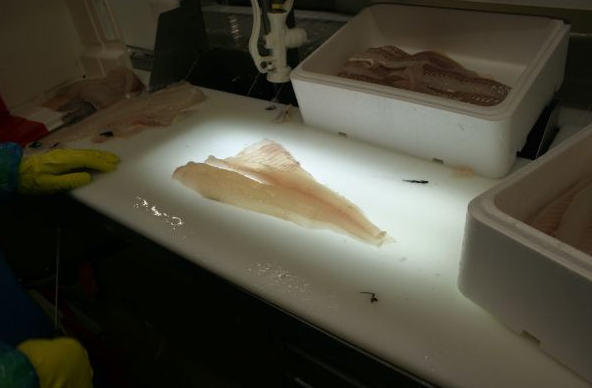
\includegraphics[scale=0.5]{Table_mirage.png}
   \caption {Détection des larves d'Anisakidés en industrie sur table de mirage classique. [Réf 7]}
\end{figure}

\subsection{ la méthode du mirage au laser:}

De nombreuses alternatives ont été tentées pour détecter les parasites dans les filets  essentiellement  par exemple le mirage au laser,
\subsection{ la méthode des rayons X :}
 les rayons X,


\subsection{La méthode du  microscope au scanner acoustique :}
le microscope au scanner acoustique (SLAM).



\section {Les  méthode destructrices de détection des parasites dans les filets de poissons :}
\subsection{La méthode des rayons UV :}

 \paragraph La méthode utilisant les rayons UV pour la détection des parasites dans les poissons était l’objet de plusieurs expériences.
 \paragraph De prime abord il convient de mettre en exergue les résultats d’une étude, sur laquelle se base le présent chapitre, faite par le laboratoire UK National Reference Laboratory sous le thème « Detection of Anisakidae larvae in fish fillets using ultraviolet transillumination (UVT) ». 
\paragraph En effet, les échantillons de poissons utilisé durant l’expérience peuvent être reçus sous forme de poisson entier ou sous forme de filets ou de tissus pré-préparés. Après les échantillons sont numérotés et ceux qui n’ont pas étaient traités sont immédiatement conservés dans un réfrigérateur pour un maximum de 48 heures. Durant l’expérience,  les filets sont traités sur une  table UV transilluminateur et examinés en utilisant la lumière UV.
\paragraph Les larves d'Anisakidae sont fluorescentes sous forme de taches blanches ou de vers individuels (Comme montré dans l'image N..). Les larves peuvent être, ainsi, enlevées par les ouvriers.
\begin{figure}[!h]
   \center
   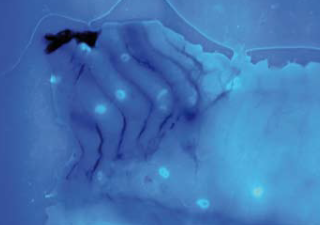
\includegraphics[scale=0.5]{UV.png}
   \caption {Anisakis encapsulé dans un filet de poisson, sous illumination avec une source de lumière ultraviolette. Les parasites individuels apparaissent sous forme d'inclusions lumineuses / fluorescentes dans la chair (image de Wootten et Bron, 2008). [Réf 2]}
\end{figure}
\paragraph Il est à préciser que les rayons sont dommageables pour les yeux d’où la nécessite d’assurer la protection appropriée et prendre les mesures et précautions adéquates. [Réf 3]
\paragraph Par ailleurs, une autre étude a été effectué par Karl, H. Leinemann, en 1993 et publiée sous le thèmes «  fast and quantitative detection method for nematodes in fish fillets and fishery products » vise à trouver une alternative pour la technique de mirage, et ce, afin d’améliorer le taux de détection des nématodes. En effet, L'efficacité de la technique de mirage est limitée par la faible pénétration de la lumière blanche dans le muscle du poisson.
\paragraph Les résultats de cette étude montrent que le taux des parasites détectés sont compris entre 52\% et 98\%, selon l’échantillon utilisé du poisson.
\paragraph Par ailleurs, une expérience faite par « Gaetano Vitale Celano, Antonello Paparella, Armida Fransvea, Claudia Balzaretti, and Giuseppe Celano» dont les résultats les conditions et les résultats sont détaillées dans cette partie.[réf5]
\paragraph En effet, l’expérience a été effectuée sur 23 échantillons de poissons appartenant à sept espèces différentes qui sont illustrés dans le tableau de la figure N
\begin{figure}[!h]
   \center
   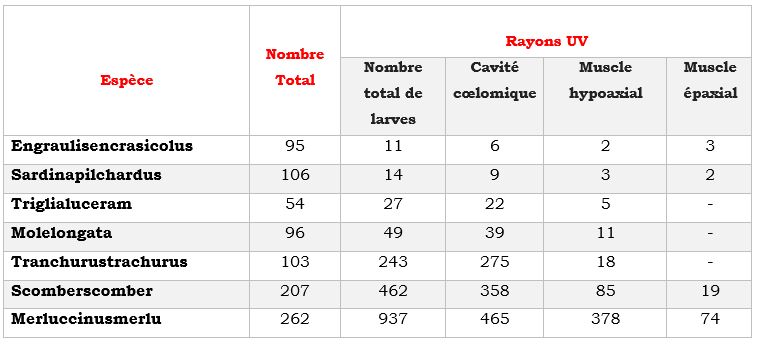
\includegraphics[scale=0.5]{Tableau01.png}
   \caption {Répartition des larves d'anisakidae dans différentes régions anatomiques de sept espèces de poissons). [Réf 2]}
\end{figure}

\paragraph Pour la transillumination UV a été effectuée comme suit: 
\begin{itemize}
\item   solution saline (1: 5 w / v) à 30 ° C a été ajouté à des chantillons de poisson, qui ont ensuite été homogénéisés dans un stomacher pendant 1 à 2 minutes.
\item l'homogénat a été pressé à couche mince de 5 mm et examiné sous lumière UV à 366 nm dans une pièce sombre. Dans de telles conditions de fonctionnement, les larves restent intactes.
\end{itemize} 
Les résultat obtenus grâce à ces deux méthodes : l’observation directe et la transillumination UV sont consignés dans le tableau ci-dessous.  
\paragraph l'analyse des résultats obtenus comme suit:
\begin{itemize}
\item En Transillumination UV, les larves d'une taille de 1 à 3 cm étaient fluorescents blanc pourrait être facilement différencié des fibres musculaires des poissons.
\item  	Dans un grand nombre d'échantillons les nématodes se déplaçaient activement et étaient clairement visibles sous la transillumination UV.
 \item	Le tableau montre la répartition des échantillons positifs dans la différente région anatomique des sept espèces de poissons, analysé par la méthode UV. Les données suggèrent que le degré d'infestation de la cavité cœlomique n'est pas en corrélation avec le degré d'infestation et localisation dans le muscle, mais peut être liée à des espèces de poissons. Dans cette étude, la récupération des tissus musculaires nettement plus élevé dans les échantillons analysés par transillumination UV. La même méthode peut également être utilisée pour distinguer les larves viables des larves mortes en colorant les larves avec plusieurs colorants ou en ajoutant du chlorure de tétrazolium . 
\end{itemize} 
\subsection {La méthode de la digestion pepsique:}
\newpage

\end{document}
